\section{Results and comparison}
\label{sec:results}
We evaluate our library in several scenarios. Furthermore, because Filib/Filib++ is the only library which is always correct when transcendental functions are involved \cite{tang2022}, we compare TIGHT with this representative of the state of the art.

All experiments were timed single-threaded on a cluster equipped with Intel Xeon Gold 6430 CPUs and 64GB of RAM.
The compiler used is GCC version 13.3.0 on Ubuntu.

\subsection{Benchmark comparison}
We start by comparing the execution times and average interval width of single functions in TIGHT and Filib++.
To compute the width, for each operation we select one or two singleton input intervals that lie inside the function domain, and compute the number of floating point values between the lower and upper ends of the computed interval (plus one); a width of 1 ULP (or 0, in the case of an exactly representable output) corresponds to a correctly rounded result.
To get timings, we call each function one million times; to prevent the compiler from optimizing calls, and to evaluate the timing on non-singleton intervals, we perturb the input interval at each iteration by enlarging it by an ULP on both sides, and sum the upper and lower bound of each result to a dummy accumulator.
Note that some operations are omitted for Filib++ as they are not supported by the library.

\clearpage
\onecolumn
\begingroup

\tiny
\begin{longtable}{lrrrrrrrrr}
\hline
& Filib & Boost & FL++ NS & FL++ ND & FL++ NOG & FL++ Mul & FL++ PS & TIGHT & FP baseline \\
\hline
ADDITION & 139.841000 & 451.849000 & 77.454000 & 56.244000 & 16.264000 & 46.557000 & 58.725000 & 5.904000 & 5.912000 \\
SUBTRACTION & 135.853000 & 451.776000 & 77.444000 & 56.186000 & 16.295000 & 40.737000 & 58.831000 & 5.914000 & 5.911000 \\
MULTIPLICATION & 153.026000 & 454.497000 & 80.465000 & 58.602000 & 17.472000 & 64.090000 & 86.292000 & 11.230000 & 5.898000 \\
DIVISION & 148.818000 & 448.056000 & 98.105000 & 74.635000 & 37.021000 & 61.618000 & 82.163000 & 47.171000 & 11.826000 \\
SQUARE ROOT & 159.648000 & 447.951000 & 79.588000 & 63.828000 & 46.856000 & 60.580000 & 96.586000 & 35.396000 & 23.587000 \\
EXPONENTIAL & 257.656000 & 449.746000 & 254.173000 & 251.163000 & 205.657000 & 219.957000 & 246.876000 & 178.049000 & 57.764000 \\
SIN & 289.798000 & 1453.097000 & 327.376000 & 324.451000 & 207.906000 & 220.579000 & 233.763000 & 1971.934000 & 317.734000 \\
COS & 288.131000 & 1304.546000 & 324.974000 & 321.932000 & 207.339000 & 221.081000 & 230.165000 & 1943.731000 & 321.314000 \\
ARITHMETIC EXPRESSION 1 & 800.244000 & 2238.724000 & 569.425000 & 506.251000 & 229.616000 & 606.002000 & 757.993000 & 293.389000 & 58.910000 \\
ARITHMETIC EXPRESSION 2 & 1139.821000 & 3363.927000 & 718.223000 & 562.186000 & 175.775000 & 713.381000 & 863.089000 & 190.415000 & 47.126000 \\
ARITHMETIC EXPRESSION 3 & 1471.388000 & 4256.047000 & 998.436000 & 831.644000 & 458.746000 & 1124.630000 & 1325.309000 & 432.067000 & 70.696000 \\
ARITHMETIC EXPRESSION 4 & 3024.144000 & 9191.820000 & 1913.025000 & 1469.517000 & 585.462000 & 2044.504000 & 3184.462000 & 459.122000 & 94.246000 \\
ARITHMETIC EXPRESSION 5 & 2119.622000 & 6502.706000 & 1393.962000 & 1059.133000 & 367.301000 & 1411.076000 & 2217.277000 & 383.853000 & 94.231000 \\
ARITHMETIC EXPRESSION 6 & 1101.514000 & 3366.891000 & 687.291000 & 545.948000 & 158.213000 & 661.872000 & 883.903000 & 139.138000 & 23.585000 \\
ARITHMETIC EXPRESSION 7 & 727.897000 & 2243.477000 & 475.341000 & 359.346000 & 108.662000 & 401.904000 & 515.303000 & 142.828000 & 35.334000 \\
ARITHMETIC EXPRESSION 8 & 769.365000 & 2240.706000 & 501.354000 & 409.604000 & 128.150000 & 481.864000 & 564.428000 & 164.013000 & 35.331000 \\
ARITHMETIC EXPRESSION 9 & 3531.364000 & 10761.818000 & 2359.372000 & 1799.626000 & 699.956000 & 2391.969000 & 3727.499000 & 664.133000 & 164.909000 \\
ARITHMETIC EXPRESSION 10 & 1373.598000 & 4270.300000 & 907.073000 & 721.146000 & 199.894000 & 838.060000 & 1163.332000 & 237.028000 & 58.922000 \\
RANDOM EXPRESSION 1 & 1827.720000 & 6615.070000 & 1779.349000 & 1609.323000 & 1542.162000 & 1642.973000 & 1870.718000 & 6340.366000 & 1015.198000 \\
RANDOM EXPRESSION 2 & 1110.558000 & 1574.543000 & 1207.523000 & 1209.263000 & 1202.284000 & 1211.369000 & 1241.036000 & 789.165000 & 274.175000 \\
RANDOM EXPRESSION 3 & 2564.935000 & 9867.541000 & 2537.120000 & 2239.824000 & 1853.468000 & 2204.140000 & 2587.499000 & 8508.530000 & 1236.388000 \\
RANDOM EXPRESSION 4 & 2493.733000 & 9065.295000 & 2429.218000 & 2193.551000 & 1959.358000 & 2149.981000 & 2358.275000 & 7401.421000 & 1053.076000 \\
RANDOM EXPRESSION 5 & 4295.013000 & 18143.857000 & 4302.392000 & 3851.088000 & 3412.519000 & 3760.806000 & 4273.319000 & 16603.437000 & 3267.921000 \\
RANDOM EXPRESSION 6 & 7123.256000 & 32280.897000 & 6643.304000 & 6209.411000 & 4621.778000 & 5985.760000 & 7125.158000 & 29410.590000 & 5601.662000 \\
RANDOM EXPRESSION 7 & 3380.392000 & 11034.476000 & 3399.323000 & 3058.806000 & 2786.271000 & 3095.534000 & 3374.356000 & 11130.759000 & 1734.586000 \\
RANDOM EXPRESSION 8 & 1311.223000 & 4473.228000 & 1187.424000 & 1168.751000 & 1161.100000 & 1213.181000 & 1331.393000 & 6055.558000 & 1215.196000 \\
RANDOM EXPRESSION 9 & 3400.103000 & 10210.072000 & 3254.755000 & 3225.024000 & 3226.479000 & 3289.355000 & 3422.299000 & 11014.137000 & 1435.637000 \\
RANDOM EXPRESSION 10 & 4138.037000 & 17332.834000 & 4199.233000 & 3891.382000 & 2984.560000 & 3604.736000 & 4267.214000 & 18873.356000 & 2856.765000 \\
rigidBody2 & 1096.688000 & 3367.143000 & 633.011000 & 454.095000 & 151.639000 & 813.494000 & 830.272000 & 81.743000 & 12.110000 \\
triangle11 & 1339.602000 & 4491.835000 & 1060.539000 & 819.971000 & 275.963000 & 668.278000 & 906.220000 & 95.955000 & 23.643000 \\
sine & 1279.160000 & 4261.529000 & 893.492000 & 702.348000 & 388.753000 & 971.968000 & 1101.282000 & 116.442000 & 35.364000 \\
sum & 603.018000 & 2022.259000 & 344.715000 & 231.917000 & 28.484000 & 202.413000 & 306.228000 & 17.685000 & 13.274000 \\
test05nonlin1, r4 & 337.751000 & 1141.695000 & 232.326000 & 193.339000 & 41.939000 & 153.593000 & 178.452000 & 51.607000 & 12.886000 \\
hartman3 & 4712.450000 & 15262.228000 & 4173.571000 & 3395.213000 & 1697.997000 & 3611.646000 & 5104.652000 & 1064.881000 & 250.838000 \\
NMSE example 3.5 & 515.136000 & 1478.805000 & 491.804000 & 354.802000 & 277.643000 & 333.407000 & 445.790000 & 261.077000 & 120.126000 \\
Shoelace formula & 962.584000 & 2928.785000 & 534.187000 & 392.263000 & 138.700000 & 612.959000 & 720.627000 & 64.175000 & 14.922000 \\
NMSE example 3.10 & 551.913000 & 1348.582000 & 578.566000 & 420.741000 & 299.711000 & 376.984000 & 425.219000 & 815.674000 & 123.662000 \\
xbyxy & 202.976000 & 673.115000 & 156.073000 & 108.681000 & 37.741000 & 68.940000 & 122.748000 & 47.172000 & 11.819000 \\
NMSE section 3.11 & 594.957000 & 1129.898000 & 544.280000 & 533.606000 & 429.692000 & 500.523000 & 552.525000 & 342.734000 & 124.125000 \\
NMSE problem 3.3.1 & 393.005000 & 1138.265000 & 236.223000 & 185.712000 & 56.550000 & 185.663000 & 201.172000 & 24.311000 & 24.309000 \\
floudas2 & 138.222000 & 454.552000 & 77.722000 & 55.966000 & 16.183000 & 53.964000 & 58.758000 & 5.910000 & 5.893000 \\
test03nonlin2 & 274.542000 & 899.087000 & 201.572000 & 144.665000 & 41.662000 & 110.584000 & 143.203000 & 47.256000 & 11.801000 \\
nonlin2 & 518.287000 & 1793.875000 & 356.922000 & 277.021000 & 65.980000 & 302.369000 & 301.113000 & 58.751000 & 11.958000 \\
Complex sine and cosine & 874.427000 & 2574.310000 & 981.011000 & 848.995000 & 633.686000 & 734.288000 & 814.541000 & 2327.376000 & 401.627000 \\
floudas & 134.963000 & 451.753000 & 77.556000 & 56.111000 & 16.277000 & 32.403000 & 58.207000 & 5.916000 & 5.892000 \\
NMSE problem 3.4.2 & 1248.118000 & 3148.093000 & 1388.299000 & 1274.505000 & 756.863000 & 1107.437000 & 1240.167000 & 641.644000 & 177.688000 \\
NMSE example 3.8 & 743.097000 & 2019.136000 & 655.366000 & 609.324000 & 305.196000 & 453.241000 & 582.945000 & 812.049000 & 120.653000 \\
polarToCarthesian, x & 397.000000 & 1572.892000 & 466.554000 & 335.737000 & 223.962000 & 286.343000 & 323.319000 & 1016.368000 & 81.874000 \\
turbine1 & 1012.643000 & 3370.635000 & 644.964000 & 472.508000 & 116.244000 & 621.345000 & 680.219000 & 116.815000 & 24.217000 \\
triangle9 & 1337.699000 & 4491.263000 & 1059.422000 & 819.973000 & 275.852000 & 666.640000 & 895.069000 & 95.963000 & 23.669000 \\
sineOrder3 & 417.451000 & 1347.220000 & 233.925000 & 158.511000 & 25.356000 & 233.001000 & 291.788000 & 26.015000 & 5.934000 \\
doppler3 & 852.926000 & 2695.586000 & 512.794000 & 367.447000 & 67.302000 & 519.224000 & 509.392000 & 49.044000 & 11.826000 \\
triangle1 & 1343.976000 & 4491.789000 & 1064.973000 & 819.938000 & 276.008000 & 687.754000 & 896.190000 & 95.991000 & 23.654000 \\
NMSE p42, negative & 733.592000 & 2019.511000 & 474.269000 & 397.573000 & 134.240000 & 467.709000 & 532.497000 & 96.133000 & 30.116000 \\
matrixDeterminant2 & 1335.914000 & 4037.783000 & 768.697000 & 590.954000 & 291.377000 & 994.170000 & 1151.122000 & 127.204000 & 17.702000 \\
delta & 2363.775000 & 8071.711000 & 1487.744000 & 1069.958000 & 368.422000 & 1623.485000 & 2516.267000 & 201.618000 & 35.574000 \\
test06sums4, sum1 & 276.214000 & 899.933000 & 154.370000 & 109.818000 & 16.670000 & 70.498000 & 116.089000 & 5.911000 & 6.271000 \\
sec4-example & 510.909000 & 1792.815000 & 358.227000 & 276.106000 & 64.924000 & 291.070000 & 299.062000 & 58.110000 & 11.850000 \\
logexp & 571.539000 & 900.015000 & 429.090000 & 422.216000 & 406.535000 & 470.908000 & 523.480000 & 608.036000 & 101.801000 \\
NMSE problem 3.3.5 & 613.752000 & 2814.852000 & 654.772000 & 640.610000 & 411.896000 & 474.869000 & 534.066000 & 3917.989000 & 645.331000 \\
NMSE example 3.3 & 624.144000 & 3115.015000 & 659.109000 & 644.230000 & 420.507000 & 481.649000 & 535.004000 & 3984.539000 & 639.393000 \\
kepler0 & 934.094000 & 3374.042000 & 591.144000 & 410.800000 & 96.445000 & 446.641000 & 690.757000 & 68.643000 & 12.998000 \\
triangle5 & 1330.043000 & 4491.454000 & 1054.046000 & 819.945000 & 275.962000 & 679.206000 & 897.956000 & 95.985000 & 23.634000 \\
bspline3 & 349.558000 & 896.634000 & 170.890000 & 132.328000 & 23.763000 & 149.554000 & 151.591000 & 25.208000 & 11.814000 \\
predatorPrey & 517.708000 & 1797.241000 & 362.751000 & 264.453000 & 71.540000 & 295.467000 & 315.223000 & 75.174000 & 23.547000 \\
turbine3 & 1078.464000 & 3374.784000 & 657.901000 & 473.523000 & 115.918000 & 671.678000 & 731.489000 & 120.067000 & 24.374000 \\
triangle7 & 1333.909000 & 4491.519000 & 1060.567000 & 820.037000 & 275.935000 & 678.737000 & 904.532000 & 95.977000 & 23.640000 \\
doppler1 & 856.010000 & 2694.662000 & 512.790000 & 367.413000 & 67.356000 & 511.259000 & 508.052000 & 49.022000 & 11.824000 \\
triangle3 & 1343.285000 & 4491.633000 & 1059.280000 & 820.024000 & 275.915000 & 675.874000 & 895.355000 & 95.984000 & 23.662000 \\
Rump's example, C & 2473.162000 & 8509.362000 & 1663.972000 & 1315.420000 & 759.647000 & 2049.098000 & 2535.792000 & 133.600000 & 18.490000 \\
exp1x & 419.860000 & 898.201000 & 472.654000 & 303.216000 & 233.508000 & 308.834000 & 361.977000 & 173.688000 & 52.859000 \\
NMSE problem 3.4.4 & 815.684000 & 1799.601000 & 753.586000 & 631.378000 & 563.758000 & 689.865000 & 822.923000 & 388.001000 & 141.606000 \\
delta4 & 1133.072000 & 3824.396000 & 680.522000 & 464.514000 & 100.704000 & 603.177000 & 910.545000 & 84.924000 & 14.717000 \\
instantaneousCurrent & 4488.761000 & 16970.875000 & 4069.743000 & 3347.207000 & 1772.621000 & 3921.790000 & 4572.856000 & 3542.066000 & 249.317000 \\
NMSE problem 3.2.1, negative & 580.000000 & 1575.099000 & 391.866000 & 343.297000 & 141.013000 & 366.826000 & 388.945000 & 95.234000 & 30.114000 \\
kepler2 & 2253.051000 & 8074.229000 & 1476.404000 & 1055.691000 & 299.644000 & 1350.289000 & 2307.827000 & 202.517000 & 31.426000 \\
NMSE problem 3.3.3 & 596.981000 & 1801.427000 & 388.592000 & 272.221000 & 84.582000 & 291.734000 & 353.846000 & 36.415000 & 36.155000 \\
azimuth & 2280.088000 & 9580.675000 & 2244.388000 & 1913.964000 & 1623.961000 & 1893.445000 & 2035.415000 & 7440.727000 & 557.777000 \\
NMSE problem 3.3.7 & 598.215000 & 1131.234000 & 612.145000 & 515.712000 & 410.170000 & 490.731000 & 563.524000 & 356.303000 & 126.512000 \\
i6 & 348.473000 & 1647.079000 & 341.872000 & 337.572000 & 222.369000 & 243.379000 & 287.750000 & 1633.076000 & 85.102000 \\
NMSE example 3.9 & 552.721000 & 1726.968000 & 596.867000 & 556.534000 & 289.913000 & 391.215000 & 460.772000 & 1264.309000 & 339.103000 \\
NMSE section 3.5 & 398.016000 & 898.768000 & 486.733000 & 303.016000 & 245.139000 & 300.453000 & 367.014000 & 197.396000 & 55.691000 \\
hypot & 342.477000 & 1122.022000 & 263.823000 & 238.321000 & 91.797000 & 224.506000 & 236.291000 & 47.483000 & 23.592000 \\
test04dqmom9 & 2386.646000 & 7176.255000 & 1458.446000 & 1147.777000 & 541.147000 & 1792.461000 & 2241.113000 & 222.694000 & 36.870000 \\
nonlin1 & 204.094000 & 673.566000 & 154.107000 & 108.823000 & 37.646000 & 68.386000 & 122.449000 & 47.215000 & 11.817000 \\
NMSE example 3.4 & 664.564000 & 2980.073000 & 661.015000 & 624.384000 & 435.720000 & 515.363000 & 550.968000 & 3860.527000 & 631.596000 \\
hartman6 & 8441.579000 & 28732.496000 & 6675.589000 & 5234.865000 & 2195.664000 & 6219.582000 & 9146.217000 & 1425.817000 & 312.680000 \\
carthesianToPolar, radius & 340.186000 & 1122.005000 & 262.460000 & 239.171000 & 87.975000 & 199.452000 & 216.425000 & 47.469000 & 23.595000 \\
triangle & 1355.984000 & 4491.370000 & 1064.677000 & 819.935000 & 275.928000 & 691.038000 & 901.196000 & 96.010000 & 23.636000 \\
jetEngine & 4359.431000 & 14353.908000 & 2896.103000 & 2259.655000 & 961.222000 & 3185.314000 & 4501.869000 & 290.648000 & 32.992000 \\
sqroot & 944.149000 & 3370.391000 & 612.010000 & 432.251000 & 109.613000 & 635.199000 & 590.473000 & 91.940000 & 16.391000 \\
triangle12 & 1343.855000 & 4491.469000 & 1062.189000 & 819.967000 & 275.913000 & 668.453000 & 923.339000 & 95.945000 & 23.652000 \\
triangle10 & 1343.627000 & 4491.394000 & 1060.932000 & 819.955000 & 275.905000 & 657.708000 & 895.633000 & 96.001000 & 23.668000 \\
turbine2 & 787.646000 & 2468.374000 & 485.223000 & 355.833000 & 83.628000 & 523.906000 & 568.031000 & 92.648000 & 13.073000 \\
triangle2 & 1349.661000 & 4491.501000 & 1060.174000 & 819.947000 & 275.856000 & 658.290000 & 889.431000 & 96.068000 & 23.639000 \\
rigidBody1 & 499.257000 & 1571.369000 & 277.324000 & 192.437000 & 33.012000 & 275.614000 & 295.456000 & 27.934000 & 6.714000 \\
NMSE problem 3.4.1 & 499.820000 & 1935.497000 & 495.778000 & 445.141000 & 234.839000 & 348.744000 & 393.001000 & 1937.419000 & 323.871000 \\
exp1xlog & 861.737000 & 1372.868000 & 839.657000 & 669.773000 & 658.511000 & 719.369000 & 771.246000 & 768.945000 & 176.738000 \\
Complex square root & 677.775000 & 2022.524000 & 478.818000 & 448.335000 & 193.064000 & 444.889000 & 523.104000 & 80.550000 & 40.673000 \\
carthesianToPolar, theta & 369.999000 & 1063.295000 & 478.198000 & 270.977000 & 190.656000 & 240.149000 & 286.038000 & 395.114000 & 67.595000 \\
NMSE example 3.7 & 346.028000 & 673.768000 & 269.469000 & 263.258000 & 215.692000 & 254.656000 & 307.312000 & 181.984000 & 55.634000 \\
floudas3 & 446.175000 & 1347.691000 & 232.976000 & 156.858000 & 23.549000 & 211.433000 & 264.065000 & 17.055000 & 5.896000 \\
NMSE example 3.6 & 575.899000 & 1571.854000 & 408.961000 & 383.614000 & 149.620000 & 336.309000 & 363.886000 & 94.401000 & 61.769000 \\
i4 & 306.219000 & 899.382000 & 225.286000 & 131.355000 & 51.645000 & 127.900000 & 197.492000 & 36.702000 & 23.587000 \\
test02sum8 & 553.056000 & 1797.845000 & 304.836000 & 208.652000 & 25.876000 & 173.014000 & 289.805000 & 11.815000 & 11.782000 \\
triangle6 & 1340.512000 & 4491.380000 & 1065.315000 & 819.995000 & 275.932000 & 684.508000 & 897.417000 & 96.035000 & 23.652000 \\
carbonGas & 633.969000 & 2063.988000 & 394.711000 & 292.047000 & 72.406000 & 296.220000 & 461.252000 & 42.795000 & 13.133000 \\
sphere & 708.084000 & 3291.394000 & 668.765000 & 637.000000 & 393.829000 & 551.753000 & 617.975000 & 2053.451000 & 116.283000 \\
test01sum3 & 600.117000 & 2022.147000 & 344.752000 & 231.906000 & 28.469000 & 196.147000 & 289.398000 & 17.683000 & 13.268000 \\
test05nonlin1, test2 & 208.727000 & 678.465000 & 155.104000 & 109.365000 & 38.017000 & 73.359000 & 124.173000 & 11.770000 & 11.786000 \\
kepler1 & 1534.837000 & 5387.201000 & 965.331000 & 696.391000 & 166.707000 & 946.730000 & 1624.203000 & 118.510000 & 20.213000 \\
NMSE example 3.1 & 424.877000 & 1122.665000 & 247.424000 & 167.236000 & 123.937000 & 238.997000 & 232.539000 & 71.246000 & 37.569000 \\
matrixDeterminant & 1306.568000 & 4040.408000 & 768.910000 & 590.688000 & 276.258000 & 997.373000 & 1157.617000 & 124.680000 & 17.704000 \\
NMSE p42, positive & 717.345000 & 2019.561000 & 472.198000 & 389.439000 & 127.389000 & 469.201000 & 518.698000 & 96.015000 & 30.050000 \\
sqrtadd & 506.413000 & 1346.585000 & 319.466000 & 249.144000 & 128.995000 & 274.941000 & 296.415000 & 84.254000 & 47.154000 \\
NMSE problem 3.4.5 & 792.389000 & 2993.750000 & 876.489000 & 749.898000 & 479.788000 & 570.157000 & 642.935000 & 3235.422000 & 652.276000 \\
floudas1 & 1675.451000 & 5614.112000 & 1050.390000 & 748.274000 & 209.619000 & 1028.023000 & 1754.377000 & 90.824000 & 15.432000 \\
NMSE problem 3.3.2 & 748.989000 & 2504.716000 & 764.071000 & 752.515000 & 509.868000 & 551.905000 & 633.419000 & 2533.860000 & 652.241000 \\
intro-example & 202.243000 & 673.536000 & 154.102000 & 108.846000 & 37.650000 & 79.441000 & 122.476000 & 47.209000 & 11.798000 \\
test06sums4, sum2 & 282.668000 & 899.772000 & 154.919000 & 109.534000 & 17.039000 & 71.091000 & 110.263000 & 5.907000 & 6.622000 \\
himmilbeau & 1079.656000 & 3603.857000 & 661.332000 & 475.050000 & 137.398000 & 599.288000 & 990.714000 & 60.156000 & 8.686000 \\
NMSE problem 3.3.6 & 532.307000 & 1122.233000 & 425.726000 & 354.958000 & 277.861000 & 337.198000 & 404.582000 & 823.688000 & 120.724000 \\
intro-example-mixed & 212.109000 & 673.567000 & 154.098000 & 108.777000 & 37.672000 & 80.346000 & 122.445000 & 47.209000 & 11.787000 \\
NMSE problem 3.4.3 & 384.190000 & 1123.837000 & 497.130000 & 442.214000 & 227.765000 & 282.040000 & 348.713000 & 411.277000 & 58.651000 \\
exp1x32 & 419.900000 & 897.561000 & 475.516000 & 303.253000 & 233.530000 & 308.849000 & 362.038000 & 173.226000 & 52.684000 \\
NMSE problem 3.2.1, positive & 556.059000 & 1574.704000 & 392.185000 & 344.205000 & 123.767000 & 356.350000 & 381.967000 & 95.345000 & 30.066000 \\
polarToCarthesian, y & 403.183000 & 1733.631000 & 467.434000 & 339.948000 & 226.865000 & 283.291000 & 324.764000 & 1011.146000 & 81.761000 \\
Rump's example, FP & 2309.869000 & 7614.761000 & 1495.628000 & 1183.428000 & 651.137000 & 1936.570000 & 2352.014000 & 149.952000 & 18.556000 \\
triangle8 & 1347.005000 & 4491.694000 & 1058.567000 & 819.899000 & 275.912000 & 658.487000 & 895.219000 & 95.900000 & 23.666000 \\
verhulst & 350.615000 & 1121.993000 & 236.814000 & 190.891000 & 47.872000 & 117.664000 & 181.299000 & 64.693000 & 23.553000 \\
triangle4 & 1348.819000 & 4492.027000 & 1060.792000 & 819.955000 & 275.959000 & 660.079000 & 889.145000 & 96.004000 & 23.682000 \\
doppler2 & 844.834000 & 2695.186000 & 514.055000 & 367.496000 & 67.403000 & 530.879000 & 524.273000 & 49.006000 & 11.800000 \\
\hline
\end{longtable}

\endgroup
\clearpage
\twocolumn


\subsection{Comparison with Filib++ within MiSo}
To assess the practical effectiveness of our library, we integrate it in the software MiSo \cite{miso} which makes intensive use of interval arithmetic.
MiSo is a Python tool to generate interval-based C++ solvers with correctness guarantees, and already uses NFG for its fast interval arithmetic, albeit with no support for non-algebraic operations.
Since MiSo's architecture allows for easily switching the numeric backend, we were able to perform a side-by-side comparison of our library and Filib++ for several problems, while extending the software's support to transcendental operators.

These problems involve heavy use of trigonometric functions which, as outlined in Section \ref{}, are more expensive to compute in TIGHT than in Filib++.
However, as we shall see, TIGHT's faster handling of basic arithmetic and its smaller intervals result in faster solution times overall.

\subsubsection{CCD along non-algebraic trajectories}
\begin{figure}
	\centering
	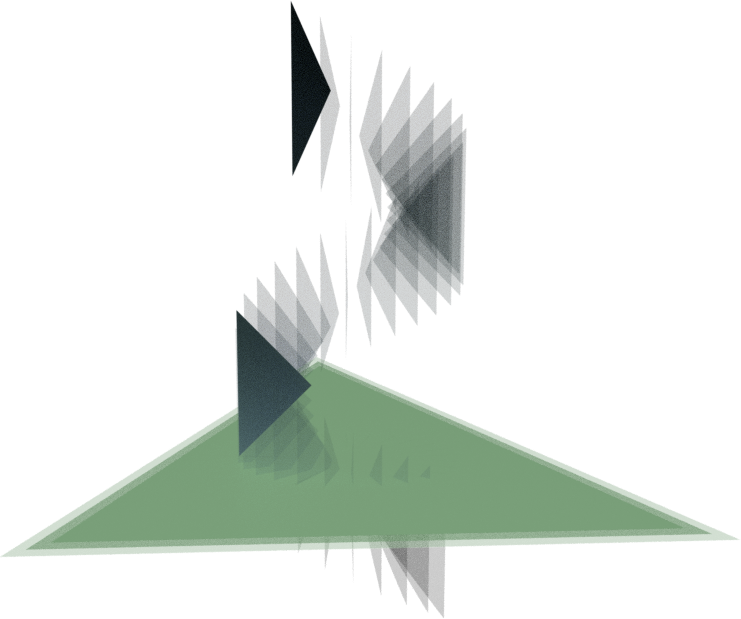
\includegraphics[width=0.8\linewidth]{fig/spiral.png}
	\caption{Test problem: \FS{caption}}
	\label{fig:tori}
\end{figure}
We consider the classical problem of continuous collision detection (CCD): given two primitives in space with some prescribed trajectory, we seek the first time in $[0,1]$ for which the primitives first come into contact, and call it $t^*$.
In practice, finding the exact value of $t^*$ may be infeasible and often unneceessary. With interval methods we instead seek an interval $T^*$ that is guaranteed to contain $t^*$ and is smaller than a user-specified precision $\delta>0$.
Then the lower bound of $T^*$ tells us a moment in time until which we can safely move the objects without collisions, and the upper bound gives a moment when collision has surely happened already.
This type of test is essential in the simulation field to guarantee that physical objects do not interpenetrate.
The difficulty of the query depends on the type of primitives, the type of trajectory, and the precision required.

Within MiSo, this is formulated as a \textsc{Minimize} problem, that is, a constrained global optimization.
In this case the optimization variables are $\{\mathbf{u}, \mathbf{v}, t\}$, where $\mathbf{u}=(u_0, u_1)$ and $\mathbf{v}=(v_0, v_1)$ are the parametric coordinates of the two primitives, and $t$ is time;
the constraints are the domain constraints $(u_0,u_1,v_0,v_1,t)\in[0,1]^5, u_0+u_1\leq1, v_0+v_1\leq1$ (which are all implicit in MiSo), and the collision constraint $d(x,y)<\epsilon$ with a small but positive $\epsilon$ (we only consider pairs of points for which collision happens);
the objective function is $t$ (we want to find the collision that happens earliest).

In our test, we consider two moving linear (i.e. flat) triangles, where one is linearly deforming (i.e. each vertex follows a linear trajectory independent of the others), while the other vertex is undergoing a rigid roto-translation, following a spiral motion.

We test the same problem with different sets of parameters, changing the speed of the rotation and the position of the other triangle. The queries implemented with TIGHT take $27$ms, $133$ms and $2.5$s respectively, versus the $127$ms, $756$ms and $13.2$s of Filib++, for a speedup of approximately $5\times$.

\subsubsection{Intersection of two parametric tori}
\begin{figure}
	\centering
	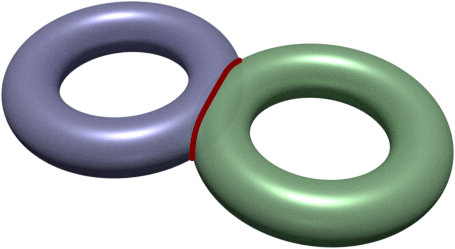
\includegraphics[width=0.8\linewidth]{fig/torusInt.png}
	\caption{Test problem: surface-surface intersection (SSI) of two parametric tori of inner radius $0.3$ and outer radius $1$, each shifted by $\pm1.1$ along the $x$ axis.}
	\label{fig:tori}
\end{figure}
Computing the intersection of parametric surfaces, also known as surface-surface intersection (SSI), is an important operation in CAD.
In our example, we want to describe the intersection locus of two tori expressed parametrically.

SSI can be formulated in MiSo as a \textsc{Solve} problem, that is, the problem of covering the set of all solutions of a constraint system within a certain tolerance.
Being a conservative method, the algorithm returns a region that is larger than the true solution, but is guaranteed to contain every point of it.

Similarly to the previous example, the optimization variables are $\{\mathbf{u}, \mathbf{v}\}$, where $\mathbf{u}=(u_0, u_1)$ and $\mathbf{v}=(v_0, v_1)$ are the parametric coordinates of the two tori;
the constraints are the domain constraints $(u_0,u_1,v_0,v_1)\in[0,1]^4$ (implicit in MiSo), and the intersection constraint $d(x,y)<\epsilon$.
This formulation gives solutions in \emph{parameter} space rather than physical space. To be precise, this formulation solves a more general version of the problem: since the parameter space is 4-dimensional, the solution is a collection of 4D boxes that describe pairs of contacting regions, up to the specified tolerance.

In both cases, the solver performs 11105 iterations and found a solution composed of 6976 4D boxes. However, the result took $136$ms to compute with TIGHT and $2186$ms with Filib++, a speedup of about $16\times$.

\MA{Forse val la pena chiarire/ribadire che sia in questo che nell'esempio precedente il problema richiede il calcolo di funzioni trascendenti.}

\subsection{Pathological cases}
Not producing tight enough intervals can have unpredictable results for seemingly easy problems. We provide two very simple examples where returning a slightly larger interval results in the program being unable to compute the result.

\begin{figure}
	
\includegraphics[width=0.4\linewidth]{fig/512x512.png}
	\centering
	\caption{An example where tighter intervals of CR functions prevent errors: when the inputs to the problem are a few ULPs away from producing pathological situations, CR minimizes error and is often able to avoid failure. Moreover, its results are machine-independent; a non-CR implementation may complete successfully on one machine but fail on another.}
	\label{fig:tori}
\end{figure}
Suppose we have a function $f(x,y)$ defined on the plane that is inversely proportional to the distance of point $(x,y)$ to a circle centered in the origin with radius 5.
Thus, we are evaluating $f(x,y) = 1/(\sqrt{x^2 + y^2}-5)$.
This type of function resembles contact potentials used in IPC physical simulations.
We want to evaluate $f$ with interval arithmetic at point $P(3+10^{-15},4+10^{-15})$, so that $P$ lies outside the sphere. Remember that, because we are using interval arithmetic, we need not fear that adding a small value leads to cancellation for very small $\epsilon$: in those cases we simply get an interval that contains the true value.
We compute this function in three ways:
\begin{itemize}
	\item with TIGHT intervals, and using the function \texttt{hypot} to compute the Euclidean distance of $P$ from the origin (which is absent in Filib++);
	\item with TIGHT intervals, using only operators which are also supported by Filib++ (all algebraic in this case);
	\item with Filib++ intervals, using the same mode as the rest of the paper.
\end{itemize}
In the first two cases, the denominator is correctly computed as positive with TIGHT and the operation returns a real interval (albeit larger in the second case, due to multiple operations being involved).
When using Filib++, the square root produces an interval with lower bound equal to the radius, resulting in a division by zero.

These are simple examples, but for more complex expressions the propagation of error can be even more dramatic. While correct rounding does not completely eliminate the issue, it reduces propagation to a minimum and makes it predictable, since each operation can introduce at most 1 ULP of error on each side.

%\clearpage
\onecolumn
\begingroup

\tiny
\begin{longtable}{lrrrrrrrrr}
\hline
& Filib & Boost & FL++ NS & FL++ ND & FL++ NOG & FL++ Mul & FL++ PS & TIGHT & FP baseline \\
\hline
ADDITION & 139.841000 & 451.849000 & 77.454000 & 56.244000 & 16.264000 & 46.557000 & 58.725000 & 5.904000 & 5.912000 \\
SUBTRACTION & 135.853000 & 451.776000 & 77.444000 & 56.186000 & 16.295000 & 40.737000 & 58.831000 & 5.914000 & 5.911000 \\
MULTIPLICATION & 153.026000 & 454.497000 & 80.465000 & 58.602000 & 17.472000 & 64.090000 & 86.292000 & 11.230000 & 5.898000 \\
DIVISION & 148.818000 & 448.056000 & 98.105000 & 74.635000 & 37.021000 & 61.618000 & 82.163000 & 47.171000 & 11.826000 \\
SQUARE ROOT & 159.648000 & 447.951000 & 79.588000 & 63.828000 & 46.856000 & 60.580000 & 96.586000 & 35.396000 & 23.587000 \\
EXPONENTIAL & 257.656000 & 449.746000 & 254.173000 & 251.163000 & 205.657000 & 219.957000 & 246.876000 & 178.049000 & 57.764000 \\
SIN & 289.798000 & 1453.097000 & 327.376000 & 324.451000 & 207.906000 & 220.579000 & 233.763000 & 1971.934000 & 317.734000 \\
COS & 288.131000 & 1304.546000 & 324.974000 & 321.932000 & 207.339000 & 221.081000 & 230.165000 & 1943.731000 & 321.314000 \\
ARITHMETIC EXPRESSION 1 & 800.244000 & 2238.724000 & 569.425000 & 506.251000 & 229.616000 & 606.002000 & 757.993000 & 293.389000 & 58.910000 \\
ARITHMETIC EXPRESSION 2 & 1139.821000 & 3363.927000 & 718.223000 & 562.186000 & 175.775000 & 713.381000 & 863.089000 & 190.415000 & 47.126000 \\
ARITHMETIC EXPRESSION 3 & 1471.388000 & 4256.047000 & 998.436000 & 831.644000 & 458.746000 & 1124.630000 & 1325.309000 & 432.067000 & 70.696000 \\
ARITHMETIC EXPRESSION 4 & 3024.144000 & 9191.820000 & 1913.025000 & 1469.517000 & 585.462000 & 2044.504000 & 3184.462000 & 459.122000 & 94.246000 \\
ARITHMETIC EXPRESSION 5 & 2119.622000 & 6502.706000 & 1393.962000 & 1059.133000 & 367.301000 & 1411.076000 & 2217.277000 & 383.853000 & 94.231000 \\
ARITHMETIC EXPRESSION 6 & 1101.514000 & 3366.891000 & 687.291000 & 545.948000 & 158.213000 & 661.872000 & 883.903000 & 139.138000 & 23.585000 \\
ARITHMETIC EXPRESSION 7 & 727.897000 & 2243.477000 & 475.341000 & 359.346000 & 108.662000 & 401.904000 & 515.303000 & 142.828000 & 35.334000 \\
ARITHMETIC EXPRESSION 8 & 769.365000 & 2240.706000 & 501.354000 & 409.604000 & 128.150000 & 481.864000 & 564.428000 & 164.013000 & 35.331000 \\
ARITHMETIC EXPRESSION 9 & 3531.364000 & 10761.818000 & 2359.372000 & 1799.626000 & 699.956000 & 2391.969000 & 3727.499000 & 664.133000 & 164.909000 \\
ARITHMETIC EXPRESSION 10 & 1373.598000 & 4270.300000 & 907.073000 & 721.146000 & 199.894000 & 838.060000 & 1163.332000 & 237.028000 & 58.922000 \\
RANDOM EXPRESSION 1 & 1827.720000 & 6615.070000 & 1779.349000 & 1609.323000 & 1542.162000 & 1642.973000 & 1870.718000 & 6340.366000 & 1015.198000 \\
RANDOM EXPRESSION 2 & 1110.558000 & 1574.543000 & 1207.523000 & 1209.263000 & 1202.284000 & 1211.369000 & 1241.036000 & 789.165000 & 274.175000 \\
RANDOM EXPRESSION 3 & 2564.935000 & 9867.541000 & 2537.120000 & 2239.824000 & 1853.468000 & 2204.140000 & 2587.499000 & 8508.530000 & 1236.388000 \\
RANDOM EXPRESSION 4 & 2493.733000 & 9065.295000 & 2429.218000 & 2193.551000 & 1959.358000 & 2149.981000 & 2358.275000 & 7401.421000 & 1053.076000 \\
RANDOM EXPRESSION 5 & 4295.013000 & 18143.857000 & 4302.392000 & 3851.088000 & 3412.519000 & 3760.806000 & 4273.319000 & 16603.437000 & 3267.921000 \\
RANDOM EXPRESSION 6 & 7123.256000 & 32280.897000 & 6643.304000 & 6209.411000 & 4621.778000 & 5985.760000 & 7125.158000 & 29410.590000 & 5601.662000 \\
RANDOM EXPRESSION 7 & 3380.392000 & 11034.476000 & 3399.323000 & 3058.806000 & 2786.271000 & 3095.534000 & 3374.356000 & 11130.759000 & 1734.586000 \\
RANDOM EXPRESSION 8 & 1311.223000 & 4473.228000 & 1187.424000 & 1168.751000 & 1161.100000 & 1213.181000 & 1331.393000 & 6055.558000 & 1215.196000 \\
RANDOM EXPRESSION 9 & 3400.103000 & 10210.072000 & 3254.755000 & 3225.024000 & 3226.479000 & 3289.355000 & 3422.299000 & 11014.137000 & 1435.637000 \\
RANDOM EXPRESSION 10 & 4138.037000 & 17332.834000 & 4199.233000 & 3891.382000 & 2984.560000 & 3604.736000 & 4267.214000 & 18873.356000 & 2856.765000 \\
rigidBody2 & 1096.688000 & 3367.143000 & 633.011000 & 454.095000 & 151.639000 & 813.494000 & 830.272000 & 81.743000 & 12.110000 \\
triangle11 & 1339.602000 & 4491.835000 & 1060.539000 & 819.971000 & 275.963000 & 668.278000 & 906.220000 & 95.955000 & 23.643000 \\
sine & 1279.160000 & 4261.529000 & 893.492000 & 702.348000 & 388.753000 & 971.968000 & 1101.282000 & 116.442000 & 35.364000 \\
sum & 603.018000 & 2022.259000 & 344.715000 & 231.917000 & 28.484000 & 202.413000 & 306.228000 & 17.685000 & 13.274000 \\
test05nonlin1, r4 & 337.751000 & 1141.695000 & 232.326000 & 193.339000 & 41.939000 & 153.593000 & 178.452000 & 51.607000 & 12.886000 \\
hartman3 & 4712.450000 & 15262.228000 & 4173.571000 & 3395.213000 & 1697.997000 & 3611.646000 & 5104.652000 & 1064.881000 & 250.838000 \\
NMSE example 3.5 & 515.136000 & 1478.805000 & 491.804000 & 354.802000 & 277.643000 & 333.407000 & 445.790000 & 261.077000 & 120.126000 \\
Shoelace formula & 962.584000 & 2928.785000 & 534.187000 & 392.263000 & 138.700000 & 612.959000 & 720.627000 & 64.175000 & 14.922000 \\
NMSE example 3.10 & 551.913000 & 1348.582000 & 578.566000 & 420.741000 & 299.711000 & 376.984000 & 425.219000 & 815.674000 & 123.662000 \\
xbyxy & 202.976000 & 673.115000 & 156.073000 & 108.681000 & 37.741000 & 68.940000 & 122.748000 & 47.172000 & 11.819000 \\
NMSE section 3.11 & 594.957000 & 1129.898000 & 544.280000 & 533.606000 & 429.692000 & 500.523000 & 552.525000 & 342.734000 & 124.125000 \\
NMSE problem 3.3.1 & 393.005000 & 1138.265000 & 236.223000 & 185.712000 & 56.550000 & 185.663000 & 201.172000 & 24.311000 & 24.309000 \\
floudas2 & 138.222000 & 454.552000 & 77.722000 & 55.966000 & 16.183000 & 53.964000 & 58.758000 & 5.910000 & 5.893000 \\
test03nonlin2 & 274.542000 & 899.087000 & 201.572000 & 144.665000 & 41.662000 & 110.584000 & 143.203000 & 47.256000 & 11.801000 \\
nonlin2 & 518.287000 & 1793.875000 & 356.922000 & 277.021000 & 65.980000 & 302.369000 & 301.113000 & 58.751000 & 11.958000 \\
Complex sine and cosine & 874.427000 & 2574.310000 & 981.011000 & 848.995000 & 633.686000 & 734.288000 & 814.541000 & 2327.376000 & 401.627000 \\
floudas & 134.963000 & 451.753000 & 77.556000 & 56.111000 & 16.277000 & 32.403000 & 58.207000 & 5.916000 & 5.892000 \\
NMSE problem 3.4.2 & 1248.118000 & 3148.093000 & 1388.299000 & 1274.505000 & 756.863000 & 1107.437000 & 1240.167000 & 641.644000 & 177.688000 \\
NMSE example 3.8 & 743.097000 & 2019.136000 & 655.366000 & 609.324000 & 305.196000 & 453.241000 & 582.945000 & 812.049000 & 120.653000 \\
polarToCarthesian, x & 397.000000 & 1572.892000 & 466.554000 & 335.737000 & 223.962000 & 286.343000 & 323.319000 & 1016.368000 & 81.874000 \\
turbine1 & 1012.643000 & 3370.635000 & 644.964000 & 472.508000 & 116.244000 & 621.345000 & 680.219000 & 116.815000 & 24.217000 \\
triangle9 & 1337.699000 & 4491.263000 & 1059.422000 & 819.973000 & 275.852000 & 666.640000 & 895.069000 & 95.963000 & 23.669000 \\
sineOrder3 & 417.451000 & 1347.220000 & 233.925000 & 158.511000 & 25.356000 & 233.001000 & 291.788000 & 26.015000 & 5.934000 \\
doppler3 & 852.926000 & 2695.586000 & 512.794000 & 367.447000 & 67.302000 & 519.224000 & 509.392000 & 49.044000 & 11.826000 \\
triangle1 & 1343.976000 & 4491.789000 & 1064.973000 & 819.938000 & 276.008000 & 687.754000 & 896.190000 & 95.991000 & 23.654000 \\
NMSE p42, negative & 733.592000 & 2019.511000 & 474.269000 & 397.573000 & 134.240000 & 467.709000 & 532.497000 & 96.133000 & 30.116000 \\
matrixDeterminant2 & 1335.914000 & 4037.783000 & 768.697000 & 590.954000 & 291.377000 & 994.170000 & 1151.122000 & 127.204000 & 17.702000 \\
delta & 2363.775000 & 8071.711000 & 1487.744000 & 1069.958000 & 368.422000 & 1623.485000 & 2516.267000 & 201.618000 & 35.574000 \\
test06sums4, sum1 & 276.214000 & 899.933000 & 154.370000 & 109.818000 & 16.670000 & 70.498000 & 116.089000 & 5.911000 & 6.271000 \\
sec4-example & 510.909000 & 1792.815000 & 358.227000 & 276.106000 & 64.924000 & 291.070000 & 299.062000 & 58.110000 & 11.850000 \\
logexp & 571.539000 & 900.015000 & 429.090000 & 422.216000 & 406.535000 & 470.908000 & 523.480000 & 608.036000 & 101.801000 \\
NMSE problem 3.3.5 & 613.752000 & 2814.852000 & 654.772000 & 640.610000 & 411.896000 & 474.869000 & 534.066000 & 3917.989000 & 645.331000 \\
NMSE example 3.3 & 624.144000 & 3115.015000 & 659.109000 & 644.230000 & 420.507000 & 481.649000 & 535.004000 & 3984.539000 & 639.393000 \\
kepler0 & 934.094000 & 3374.042000 & 591.144000 & 410.800000 & 96.445000 & 446.641000 & 690.757000 & 68.643000 & 12.998000 \\
triangle5 & 1330.043000 & 4491.454000 & 1054.046000 & 819.945000 & 275.962000 & 679.206000 & 897.956000 & 95.985000 & 23.634000 \\
bspline3 & 349.558000 & 896.634000 & 170.890000 & 132.328000 & 23.763000 & 149.554000 & 151.591000 & 25.208000 & 11.814000 \\
predatorPrey & 517.708000 & 1797.241000 & 362.751000 & 264.453000 & 71.540000 & 295.467000 & 315.223000 & 75.174000 & 23.547000 \\
turbine3 & 1078.464000 & 3374.784000 & 657.901000 & 473.523000 & 115.918000 & 671.678000 & 731.489000 & 120.067000 & 24.374000 \\
triangle7 & 1333.909000 & 4491.519000 & 1060.567000 & 820.037000 & 275.935000 & 678.737000 & 904.532000 & 95.977000 & 23.640000 \\
doppler1 & 856.010000 & 2694.662000 & 512.790000 & 367.413000 & 67.356000 & 511.259000 & 508.052000 & 49.022000 & 11.824000 \\
triangle3 & 1343.285000 & 4491.633000 & 1059.280000 & 820.024000 & 275.915000 & 675.874000 & 895.355000 & 95.984000 & 23.662000 \\
Rump's example, C & 2473.162000 & 8509.362000 & 1663.972000 & 1315.420000 & 759.647000 & 2049.098000 & 2535.792000 & 133.600000 & 18.490000 \\
exp1x & 419.860000 & 898.201000 & 472.654000 & 303.216000 & 233.508000 & 308.834000 & 361.977000 & 173.688000 & 52.859000 \\
NMSE problem 3.4.4 & 815.684000 & 1799.601000 & 753.586000 & 631.378000 & 563.758000 & 689.865000 & 822.923000 & 388.001000 & 141.606000 \\
delta4 & 1133.072000 & 3824.396000 & 680.522000 & 464.514000 & 100.704000 & 603.177000 & 910.545000 & 84.924000 & 14.717000 \\
instantaneousCurrent & 4488.761000 & 16970.875000 & 4069.743000 & 3347.207000 & 1772.621000 & 3921.790000 & 4572.856000 & 3542.066000 & 249.317000 \\
NMSE problem 3.2.1, negative & 580.000000 & 1575.099000 & 391.866000 & 343.297000 & 141.013000 & 366.826000 & 388.945000 & 95.234000 & 30.114000 \\
kepler2 & 2253.051000 & 8074.229000 & 1476.404000 & 1055.691000 & 299.644000 & 1350.289000 & 2307.827000 & 202.517000 & 31.426000 \\
NMSE problem 3.3.3 & 596.981000 & 1801.427000 & 388.592000 & 272.221000 & 84.582000 & 291.734000 & 353.846000 & 36.415000 & 36.155000 \\
azimuth & 2280.088000 & 9580.675000 & 2244.388000 & 1913.964000 & 1623.961000 & 1893.445000 & 2035.415000 & 7440.727000 & 557.777000 \\
NMSE problem 3.3.7 & 598.215000 & 1131.234000 & 612.145000 & 515.712000 & 410.170000 & 490.731000 & 563.524000 & 356.303000 & 126.512000 \\
i6 & 348.473000 & 1647.079000 & 341.872000 & 337.572000 & 222.369000 & 243.379000 & 287.750000 & 1633.076000 & 85.102000 \\
NMSE example 3.9 & 552.721000 & 1726.968000 & 596.867000 & 556.534000 & 289.913000 & 391.215000 & 460.772000 & 1264.309000 & 339.103000 \\
NMSE section 3.5 & 398.016000 & 898.768000 & 486.733000 & 303.016000 & 245.139000 & 300.453000 & 367.014000 & 197.396000 & 55.691000 \\
hypot & 342.477000 & 1122.022000 & 263.823000 & 238.321000 & 91.797000 & 224.506000 & 236.291000 & 47.483000 & 23.592000 \\
test04dqmom9 & 2386.646000 & 7176.255000 & 1458.446000 & 1147.777000 & 541.147000 & 1792.461000 & 2241.113000 & 222.694000 & 36.870000 \\
nonlin1 & 204.094000 & 673.566000 & 154.107000 & 108.823000 & 37.646000 & 68.386000 & 122.449000 & 47.215000 & 11.817000 \\
NMSE example 3.4 & 664.564000 & 2980.073000 & 661.015000 & 624.384000 & 435.720000 & 515.363000 & 550.968000 & 3860.527000 & 631.596000 \\
hartman6 & 8441.579000 & 28732.496000 & 6675.589000 & 5234.865000 & 2195.664000 & 6219.582000 & 9146.217000 & 1425.817000 & 312.680000 \\
carthesianToPolar, radius & 340.186000 & 1122.005000 & 262.460000 & 239.171000 & 87.975000 & 199.452000 & 216.425000 & 47.469000 & 23.595000 \\
triangle & 1355.984000 & 4491.370000 & 1064.677000 & 819.935000 & 275.928000 & 691.038000 & 901.196000 & 96.010000 & 23.636000 \\
jetEngine & 4359.431000 & 14353.908000 & 2896.103000 & 2259.655000 & 961.222000 & 3185.314000 & 4501.869000 & 290.648000 & 32.992000 \\
sqroot & 944.149000 & 3370.391000 & 612.010000 & 432.251000 & 109.613000 & 635.199000 & 590.473000 & 91.940000 & 16.391000 \\
triangle12 & 1343.855000 & 4491.469000 & 1062.189000 & 819.967000 & 275.913000 & 668.453000 & 923.339000 & 95.945000 & 23.652000 \\
triangle10 & 1343.627000 & 4491.394000 & 1060.932000 & 819.955000 & 275.905000 & 657.708000 & 895.633000 & 96.001000 & 23.668000 \\
turbine2 & 787.646000 & 2468.374000 & 485.223000 & 355.833000 & 83.628000 & 523.906000 & 568.031000 & 92.648000 & 13.073000 \\
triangle2 & 1349.661000 & 4491.501000 & 1060.174000 & 819.947000 & 275.856000 & 658.290000 & 889.431000 & 96.068000 & 23.639000 \\
rigidBody1 & 499.257000 & 1571.369000 & 277.324000 & 192.437000 & 33.012000 & 275.614000 & 295.456000 & 27.934000 & 6.714000 \\
NMSE problem 3.4.1 & 499.820000 & 1935.497000 & 495.778000 & 445.141000 & 234.839000 & 348.744000 & 393.001000 & 1937.419000 & 323.871000 \\
exp1xlog & 861.737000 & 1372.868000 & 839.657000 & 669.773000 & 658.511000 & 719.369000 & 771.246000 & 768.945000 & 176.738000 \\
Complex square root & 677.775000 & 2022.524000 & 478.818000 & 448.335000 & 193.064000 & 444.889000 & 523.104000 & 80.550000 & 40.673000 \\
carthesianToPolar, theta & 369.999000 & 1063.295000 & 478.198000 & 270.977000 & 190.656000 & 240.149000 & 286.038000 & 395.114000 & 67.595000 \\
NMSE example 3.7 & 346.028000 & 673.768000 & 269.469000 & 263.258000 & 215.692000 & 254.656000 & 307.312000 & 181.984000 & 55.634000 \\
floudas3 & 446.175000 & 1347.691000 & 232.976000 & 156.858000 & 23.549000 & 211.433000 & 264.065000 & 17.055000 & 5.896000 \\
NMSE example 3.6 & 575.899000 & 1571.854000 & 408.961000 & 383.614000 & 149.620000 & 336.309000 & 363.886000 & 94.401000 & 61.769000 \\
i4 & 306.219000 & 899.382000 & 225.286000 & 131.355000 & 51.645000 & 127.900000 & 197.492000 & 36.702000 & 23.587000 \\
test02sum8 & 553.056000 & 1797.845000 & 304.836000 & 208.652000 & 25.876000 & 173.014000 & 289.805000 & 11.815000 & 11.782000 \\
triangle6 & 1340.512000 & 4491.380000 & 1065.315000 & 819.995000 & 275.932000 & 684.508000 & 897.417000 & 96.035000 & 23.652000 \\
carbonGas & 633.969000 & 2063.988000 & 394.711000 & 292.047000 & 72.406000 & 296.220000 & 461.252000 & 42.795000 & 13.133000 \\
sphere & 708.084000 & 3291.394000 & 668.765000 & 637.000000 & 393.829000 & 551.753000 & 617.975000 & 2053.451000 & 116.283000 \\
test01sum3 & 600.117000 & 2022.147000 & 344.752000 & 231.906000 & 28.469000 & 196.147000 & 289.398000 & 17.683000 & 13.268000 \\
test05nonlin1, test2 & 208.727000 & 678.465000 & 155.104000 & 109.365000 & 38.017000 & 73.359000 & 124.173000 & 11.770000 & 11.786000 \\
kepler1 & 1534.837000 & 5387.201000 & 965.331000 & 696.391000 & 166.707000 & 946.730000 & 1624.203000 & 118.510000 & 20.213000 \\
NMSE example 3.1 & 424.877000 & 1122.665000 & 247.424000 & 167.236000 & 123.937000 & 238.997000 & 232.539000 & 71.246000 & 37.569000 \\
matrixDeterminant & 1306.568000 & 4040.408000 & 768.910000 & 590.688000 & 276.258000 & 997.373000 & 1157.617000 & 124.680000 & 17.704000 \\
NMSE p42, positive & 717.345000 & 2019.561000 & 472.198000 & 389.439000 & 127.389000 & 469.201000 & 518.698000 & 96.015000 & 30.050000 \\
sqrtadd & 506.413000 & 1346.585000 & 319.466000 & 249.144000 & 128.995000 & 274.941000 & 296.415000 & 84.254000 & 47.154000 \\
NMSE problem 3.4.5 & 792.389000 & 2993.750000 & 876.489000 & 749.898000 & 479.788000 & 570.157000 & 642.935000 & 3235.422000 & 652.276000 \\
floudas1 & 1675.451000 & 5614.112000 & 1050.390000 & 748.274000 & 209.619000 & 1028.023000 & 1754.377000 & 90.824000 & 15.432000 \\
NMSE problem 3.3.2 & 748.989000 & 2504.716000 & 764.071000 & 752.515000 & 509.868000 & 551.905000 & 633.419000 & 2533.860000 & 652.241000 \\
intro-example & 202.243000 & 673.536000 & 154.102000 & 108.846000 & 37.650000 & 79.441000 & 122.476000 & 47.209000 & 11.798000 \\
test06sums4, sum2 & 282.668000 & 899.772000 & 154.919000 & 109.534000 & 17.039000 & 71.091000 & 110.263000 & 5.907000 & 6.622000 \\
himmilbeau & 1079.656000 & 3603.857000 & 661.332000 & 475.050000 & 137.398000 & 599.288000 & 990.714000 & 60.156000 & 8.686000 \\
NMSE problem 3.3.6 & 532.307000 & 1122.233000 & 425.726000 & 354.958000 & 277.861000 & 337.198000 & 404.582000 & 823.688000 & 120.724000 \\
intro-example-mixed & 212.109000 & 673.567000 & 154.098000 & 108.777000 & 37.672000 & 80.346000 & 122.445000 & 47.209000 & 11.787000 \\
NMSE problem 3.4.3 & 384.190000 & 1123.837000 & 497.130000 & 442.214000 & 227.765000 & 282.040000 & 348.713000 & 411.277000 & 58.651000 \\
exp1x32 & 419.900000 & 897.561000 & 475.516000 & 303.253000 & 233.530000 & 308.849000 & 362.038000 & 173.226000 & 52.684000 \\
NMSE problem 3.2.1, positive & 556.059000 & 1574.704000 & 392.185000 & 344.205000 & 123.767000 & 356.350000 & 381.967000 & 95.345000 & 30.066000 \\
polarToCarthesian, y & 403.183000 & 1733.631000 & 467.434000 & 339.948000 & 226.865000 & 283.291000 & 324.764000 & 1011.146000 & 81.761000 \\
Rump's example, FP & 2309.869000 & 7614.761000 & 1495.628000 & 1183.428000 & 651.137000 & 1936.570000 & 2352.014000 & 149.952000 & 18.556000 \\
triangle8 & 1347.005000 & 4491.694000 & 1058.567000 & 819.899000 & 275.912000 & 658.487000 & 895.219000 & 95.900000 & 23.666000 \\
verhulst & 350.615000 & 1121.993000 & 236.814000 & 190.891000 & 47.872000 & 117.664000 & 181.299000 & 64.693000 & 23.553000 \\
triangle4 & 1348.819000 & 4492.027000 & 1060.792000 & 819.955000 & 275.959000 & 660.079000 & 889.145000 & 96.004000 & 23.682000 \\
doppler2 & 844.834000 & 2695.186000 & 514.055000 & 367.496000 & 67.403000 & 530.879000 & 524.273000 & 49.006000 & 11.800000 \\
\hline
\end{longtable}

\endgroup
\clearpage
\twocolumn

